\documentclass[border=3pt]{standalone}
\usepackage{tikz}
\usetikzlibrary{patterns}
\begin{document}
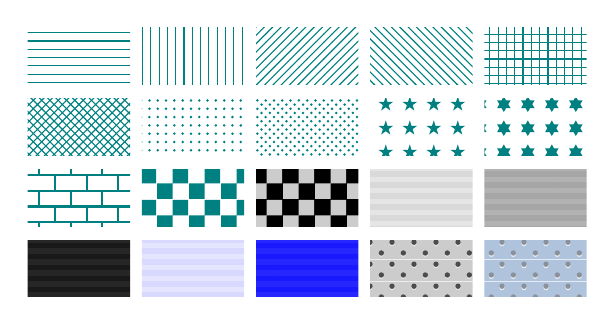
\begin{tikzpicture}
% Stock names in the order of pgfmanual-en-library-patterns.tex:56-84.
\foreach \name/\x/\y in {
  horizontal lines/0/2.7,vertical lines/1.45/2.7,north east lines/2.9/2.7,north west lines/4.35/2.7,grid/5.8/2.7,
  crosshatch/0/1.8,dots/1.45/1.8,crosshatch dots/2.9/1.8,fivepointed stars/4.35/1.8,sixpointed stars/5.8/1.8,
  bricks/0/.9,checkerboard/1.45/.9,checkerboard light gray/2.9/.9,horizontal lines light gray/4.35/.9,horizontal lines gray/5.8/.9,
  horizontal lines dark gray/0/0,horizontal lines light blue/1.45/0,horizontal lines dark blue/2.9/0,crosshatch dots gray/4.35/0,crosshatch dots light steel blue/5.8/0}{
  \fill[pattern=\name,pattern color=teal] (\x,\y) rectangle +(1.3,.72);
}
\end{tikzpicture}
\end{document}
